%%%%%%%%%%%%%%%%%%%%%%%%%%%%%%%%%%%%%%%%%%%%%%%%%%%%%%%%%%%%%%%%%%%%%%%%%%%%%%%%
%%%%%                             SETTINGS                                  %%%%
%%%%%%%%%%%%%%%%%%%%%%%%%%%%%%%%%%%%%%%%%%%%%%%%%%%%%%%%%%%%%%%%%%%%%%%%%%%%%%%%
\documentclass{article}

\usepackage{inputenc}
\usepackage[margin = 1.25in]{geometry}

\usepackage{setspace}
\onehalfspacing

\usepackage{hyperref}
\usepackage{dsfont}
\usepackage{amsmath,amssymb,dsfont,amsthm}

\usepackage{graphicx}
\usepackage{caption}
\usepackage{subcaption}
\usepackage{booktabs}

\usepackage[inline]{enumitem}
\usepackage{pdflscape}

% Default paths for figures
\usepackage{epstopdf}

\usepackage[backend = bibtex,
            style = authoryear,
            maxnames = 6,
            maxcitenames = 3,
            doi = false,
            eprint = false]{biblatex}
\addbibresource{biblio.bib}

% Bibliography
\DeclareCiteCommand{\citeyear}
	{}
	{\bibhyperref{\printdate}}
	{\multicitedelim}
	{}

% Math-related commands
\newtheorem{assu}{Assumption}
\newtheorem{prop}{Proposition}
\newtheorem{definition}{Definition}

\newcommand{\Z}{\mathcal{Z}}
\newcommand{\MW}{\underline{W}}
\newcommand{\mw}{\underline{w}}
\newcommand{\wkp}{\text{wkp}}
\newcommand{\res}{\text{res}}
\newcommand{\pre}{\text{Pre}}
\newcommand{\post}{\text{Post}}
\DeclareMathOperator{\Var}{Var}
\DeclareMathOperator{\Corr}{Corr}
\DeclareMathOperator{\Cov}{Cov}
\DeclareMathOperator{\E}{E}

%%%%%%%%%%%%%%%%%%%%%%%%%%%%%%%%%%%%%%%%%%%%%%%%%%%%%%%%%%%%%%%%%%%%%%%%%%%%%%%%
%%%%%                               TITLE                                   %%%%
%%%%%%%%%%%%%%%%%%%%%%%%%%%%%%%%%%%%%%%%%%%%%%%%%%%%%%%%%%%%%%%%%%%%%%%%%%%%%%%%

\title{Potential Outcomes and Identification for \\
       ``Minimum Wage as a Place-Based Policy''}

\author{SH}

\date{\today}

%%%%%%%%%%%%%%%%%%%%%%%%%%%%%%%%%%%%%%%%%%%%%%%%%%%%%%%%%%%%%%%%%%%%%%%%%%%%%%%%
%%%%                              STRUCTURE                                 %%%%
%%%%%%%%%%%%%%%%%%%%%%%%%%%%%%%%%%%%%%%%%%%%%%%%%%%%%%%%%%%%%%%%%%%%%%%%%%%%%%%%

\begin{document}

\maketitle

In this note we explore a potential outcomes approach for identification in 
``Minimum Wage as a Place-Based Policy: Evidence from US housing rental markets.''

\section*{Potential Outcomes Framework}

Consider the causal model for rents given by
$$r_{it}=r_{it}(\{\mw_{zt}\}_{z\in\Z})$$
where $\mw_{zt}=\ln\MW_{zt}$ for $\MW_{zt}$ the statutory MW (in dollars).
The set $\Z$ contains all ZIP codes in a closed metropolitan area.
We assume that the effects of MW across locations can be summarized in the
residence and workplace MW measures, so that
\begin{equation}\label{eq:causal_model}
    r_{it} = r_{it}(\mw_{it}^{\res}, \mw_{it}^{\wkp}) .
\end{equation}

We follow \textcite{AngristImbens1995} and define the treatment effects of 
interest as follows.
Focus on the workplace MW, and condition on a level of the residence MW.
A unit's causal response is 
$\partial r_{it}(\mw_{it}^{\res}, \mw_{it}^{\wkp})/\partial \mw_{it}^{\wkp} .$
The average causal response for the treated with dose $w$ of the workplace MW is
\begin{equation*}
    ACRT^{\wkp}(w | \mw^{\res}, w) = \frac{\partial \E\left[r_{it}(\mw^{\res}, l)
    |                           \mw^{\res}, w\right]}{\partial l} \Big|_{l=w}
\end{equation*}
and the average causal response to dose $w$ for any group is
\begin{equation*}
    ACR^{\wkp}(w | \mw^{\res}) = \frac{\partial \E\left[r_{it}(\mw^{\res}, w) \right] }{\partial w} .
\end{equation*}
We are also interested in analogous parameters for the residence MW:
\begin{equation*}
    ACRT^{\res}(w | w, \mw^{\wkp}) = \frac{\partial \E\left[r_{it}(l, \mw^{\wkp})
    |                               w, \mw^{\wkp}\right]}{\partial l} \Big|_{l=w}
\end{equation*}
and
\begin{equation*}
    ACR^{\res}(w | \mw^{\wkp}) = \frac{\partial \E\left[r_{it}(w, \mw^{\wkp}) \right] }{\partial w} .
\end{equation*}

We frame our discussion around the following policy change.

\begin{definition}[Policy change]\label{def:policy_change}
    In period $t-1$, all locations are bound by a common MW level, 
    $\MW_{i,t-1}=\MW_0$ for all $i$.
    In period $t$, the MW increases to $\MW_1>\MW_0$ in some 
    (directly treated) ZIP codes $i\in\Z_1\subset\Z$ for non-empty $\Z_1$.
    The MW levels in $t$ are then 
    $\MW_{i,t}=\MW_0$ for $i\notin\Z_1$ and
    $\MW_{i,t}=\MW_1$ for $i\in\Z_1$.
    Thus, for each $i$ the residence MW levels are
    $$
    \mw_{i,t}^{\res} = 
    \begin{cases}
        \ln \MW_1 & \text{ if } i\in\Z_1 \\
        \ln \MW_0 & \text{ if } i\notin\Z_1 
    \end{cases}
    \quad\text{ and }\quad
    \mw_{i,t-1}^{\res} = \ln \MW_0 ,
    $$
    and the workplace MW levels are computed by
    $$
    \mw_{i,t}^{\wkp} = \sum_{z\in\Z} \pi_{iz} \ln \MW_{i,t}
    $$
    where $\{\pi_{iz}\}$ are (unchanging) commuting shares.
\end{definition}

We are envisioning a policy change in which a subset of ZIP codes in a metropolitan 
area raise the level of the MW from a previously uniform level.

\begin{assu}[Parallel trends] \label{assu:PT}
    Consider the policy change in Definition \ref{def:policy_change}.
    We assume that, for all dose levels $w>\mw_0 = \ln \MW_0$,
    \begin{equation}\label{eq:PT_workplace}
        \E\left[r_{it}(\mw_0, \mw_0) - r_{i,t-1}(\mw_0, \mw_0) \big| \mw_{it}^{\wkp} = w \right] 
        = \E\left[r_{it}(\mw_0, \mw_0) - r_{i,t-1}(\mw_0, \mw_0) \big| \mw_{it}^{\wkp} = \mw_0 \right] 
    \end{equation}
    and that
    \begin{equation}\label{eq:PT_residence}
        \E\left[r_{it}(\mw_0, w) - r_{i,t-1}(\mw_0, w) \big| \mw_{it}^{\res} = \mw_1 \right] 
        = \E\left[r_{it}(\mw_0, w) - r_{i,t-1}(\mw_0, w) \big| \mw_{it}^{\res} = \mw_0 \right] .
    \end{equation}
\end{assu}

Equation \eqref{eq:PT_workplace} imposes that, conditional on not having changed
the residence MW, the counterfactual evolution of rents is the same in ZIP codes
that received any dose of the workplace MW $w$.
Equation \eqref{eq:PT_residence} imposes that, conditional on a given value of
the workplace MW, the counterfactual evolution of rents across those ZIP codes
directly treated and those not directly treated is the same.

Focusing on the workplace MW, under Assumption \ref{assu:PT}
Proposition 3 in \textcite{CallawayEtAl2021} implies that
$$
\frac{\partial \E\left[r_{it}(\mw_0, w) | \mw_{it}^{\res} = \mw_0, \mw_{it}^{\wkp} = w\right]}
     {\partial w} 
    = ACRT^{\wkp}(w | \mw_0, w) + \frac{\partial ATT^{\wkp}(w | \mw_0, l)}{\partial w} \Big|_{l = w}
$$
where $ATT^{\wkp}(w | \mw_0, w) = \E\left[r_{it}(\mw_0, w) - r_{it}(\mw_0, \mw_0) \big| \mw_{it}^{\res} = \mw_0, \mw_{it}^{\wkp} = w\right]$.
The slope of average rents with respect to the minimum wage identifies
the average causal response of interest plus a selection bias term that arises
due to differences in treatment effects across dosage leves.

Unlike the workplace MW, the residence MW experienced a discrete jump.
Then, under Assumption \ref{assu:PT} as well, 
Proposition 3 in \textcite{CallawayEtAl2021} implies
\begin{equation*}
\begin{split}
\E\left[\Delta r_{it}(\mw_1, w) | \mw_{it}^{\res} = \mw_1, \mw_{it}^{\wkp} = w\right] - \E\left[\Delta r_{it}(\mw_0, w) | \mw_{it}^{\res} = \mw_0, \mw_{it}^{\wkp} = w\right] \\
 = ACRT^{\res}(\mw_1 | \mw_1, w) + ATT^{\res}(\mw_0 | \mw_1, w) - ATT^{\res}(\mw_0 | \mw_0, w)
\end{split}
\end{equation*}
where $ATT^{\res}(\mw_1 | \mw_1, w) = \E\left[r_{it}(\mw_1, w) - r_{it}(\mw_0, w) \big| \mw_{it}^{\wkp} = w\right]$.
For a fixed level of the workplace MW, a difference in differences between
those directly treated (with $\mw^{\res}_{i,t}=\mw_1$) and
those indirectly treated (with $\mw^{\res}_{i,t-1}=\mw_0$) identifies
the causal response of interest plus a selection bias term.

As \textcite{CallawayEtAl2021} point out, the usual parallel trends assumption 
is not enough to identify the treatment effects on the treated because there may 
be selection of units to a different dosage level.
To remove these selection bias terms we could rely on a stronger version of
the parallel trends assumption 
\parencite[see Assumption 5 in][]{CallawayEtAl2021}.
However, as the authors explain in Remark 5, an alternative is to directly
assume that the selection bias terms are zero.
In this setting, we are willing to maintain this assumption.
The reason is that we are assuming an unchanging commuting structure, and
so units cannot endogenously affect the amount of dose they receive.
We think that conditioning on the level of the other MW measure makes this
assumption plausible.
We formalize these assumptions below.

\begin{assu}[No selection bias] \label{assu:no_selection}
    Consider the policy change in Definition \ref{def:policy_change}.
    We assume that
    \begin{equation*}\label{eq:PT_workplace}
        \frac{\partial ATT^{\wkp}(w | \mw_0, l)}{\partial w} \Big|_{l = w} = 0
    \end{equation*}
    and that
    \begin{equation*}\label{eq:PT_residence}
        ATT^{\res}(\mw_0 | \mw_1, w) - ATT^{\res}(\mw_0 | \mw_0, w) = 0
    \end{equation*}
\end{assu}

What comparisons does this analysis suggest?
To obtain the workplace MW we exploit the slope of the relationship
between log rents and the workplace MW, 
conditioning on units that were not directly treated.
More generally, we can compare units that received a similar amount of direct
treatment (i.e., conditioning on the residence MW).
For the residence MW we compare directly treated and directly untreated units
that have a similar level of the workplace MW.

\section*{Non-parametric identification}

Figure \ref{fig:ln_rents_mw_wkp} shows the relationship between log rents
and the workplace MW for ZIP code-months located in CBSA-months where some
MW policy changed.
Panel (a) shows the raw relation between these variables, which is increasing.
Panel (b) shows the same variables but residualized on ZIP code indicators
and 100 residence MW indicators.
Following the intuition in the previous section, we condition on the level of 
the residence MW.
The slope of this relationship is positive, and the slope is of the same
magnitude as in the main results of the paper.

Figure \ref{fig:ln_rents_mw_res} shows the relationship between log rents
and the residence MW for the same sample of ZIP codes.
Panel (a) shows that the raw correlation is positive.
Panel (b) conditions on ZIP code and 100 workplace MW indicators.
The slope turns slightly negative.

\section*{Functional form}

Assume that
$$
r_{it} = \alpha_i + \delta_t + \gamma \mw_{it}^{\res} + \beta \mw_{it}^{\wkp} + \epsilon_{it}
$$
Then, if the error term is mean independent from the MW measures, both 
Assumptions \ref{assu:PT} and \ref{assu:no_selection} hold.
Furthermore, we also have that the $ACRT$ equal the $ACR$ for any level of 
the MW measures.

\printbibliography

\clearpage
\begin{figure}[h!]
    \centering
    \caption{The relationship between log rents and the workplace MW}
    \label{fig:ln_rents_mw_wkp}

    \begin{subfigure}{.7\textwidth}
        \caption{Raw data}
        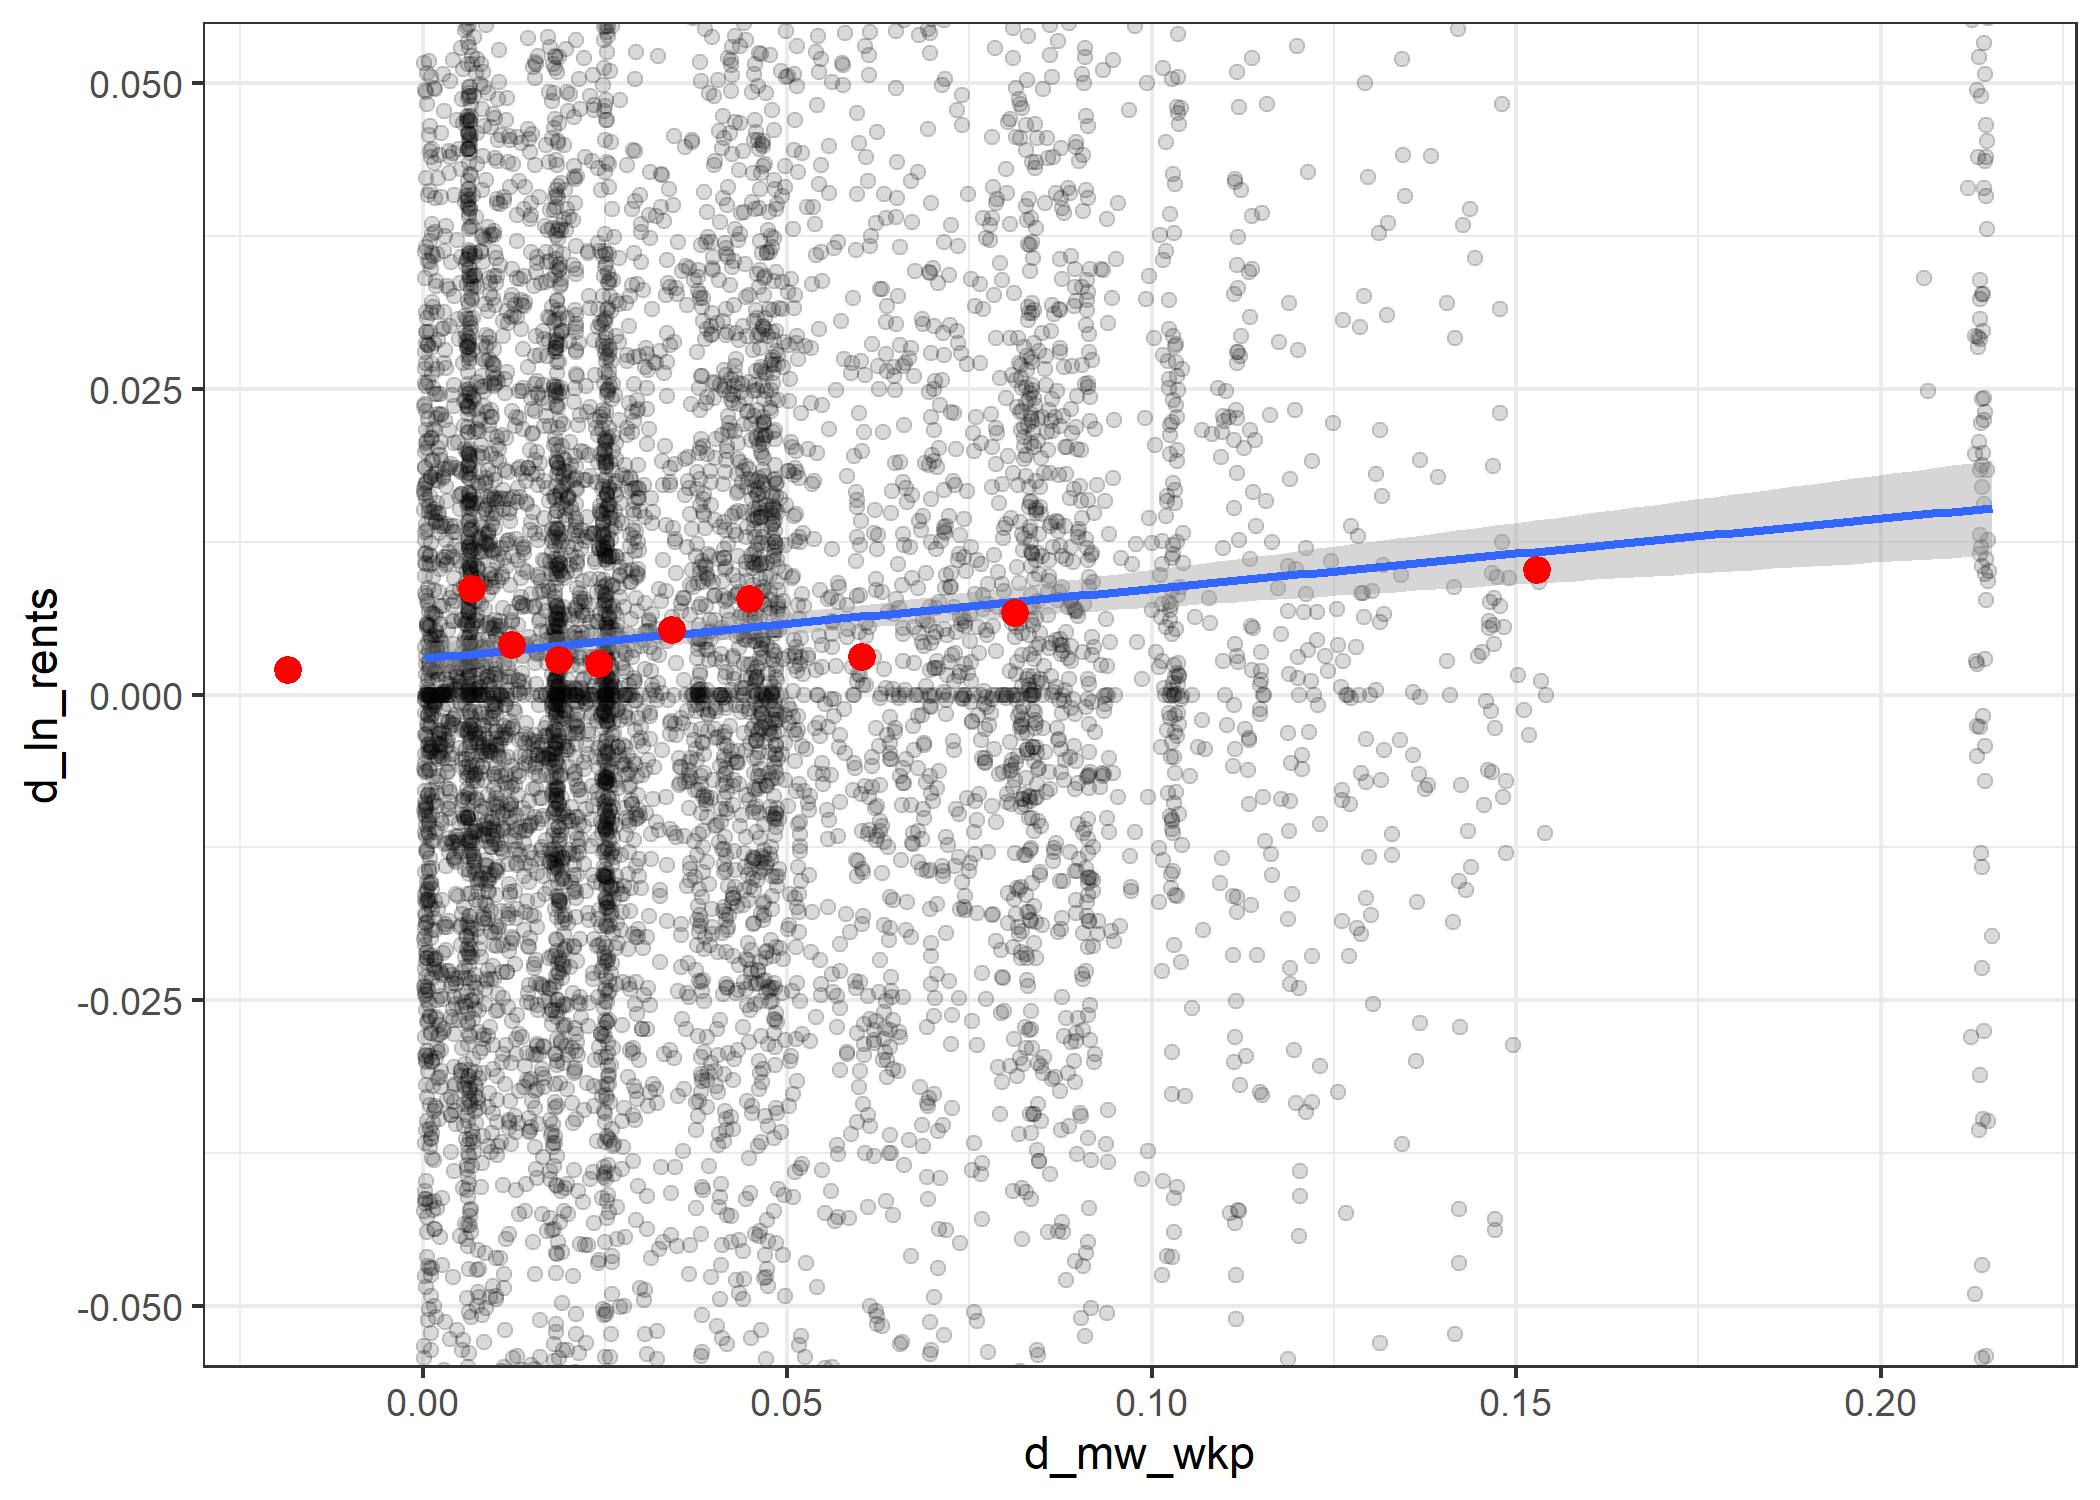
\includegraphics[width = 1\textwidth]
            {plots/cbsa_month_mw_wkp.png}
    \end{subfigure}\\
    \begin{subfigure}{.7\textwidth}
        \caption{Conditional on ZIP code and residence MW indicators}
        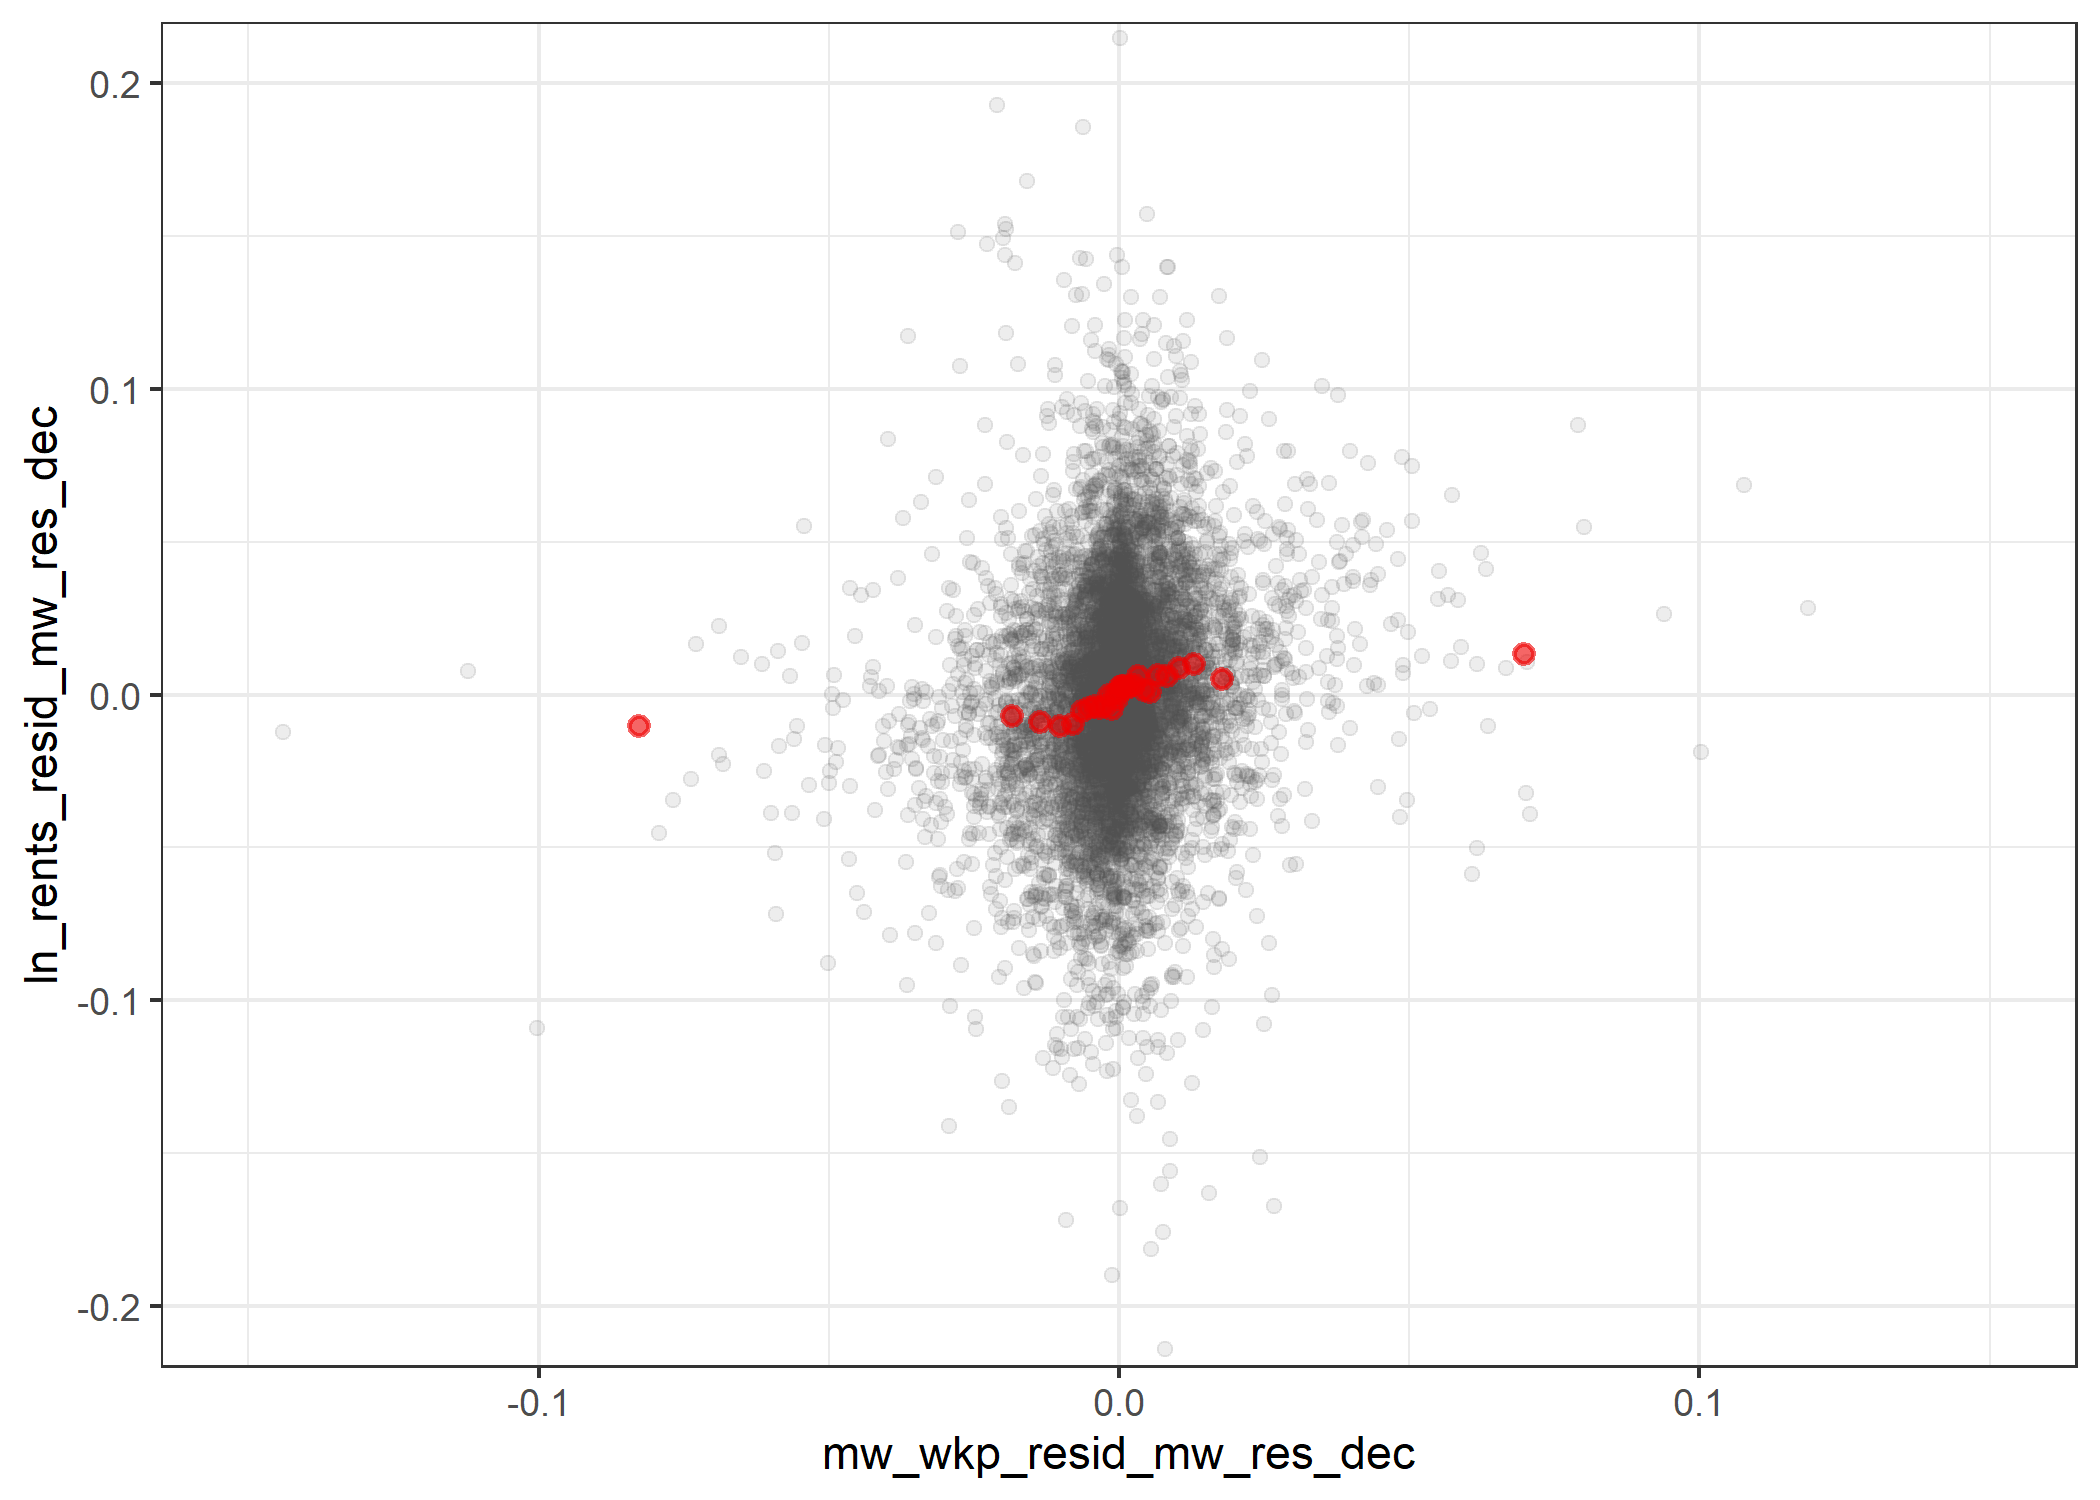
\includegraphics[width = 1\textwidth]
            {plots/cbsa_month_mw_wkp_resid_mw_res_dec.png}
    \end{subfigure}

    \begin{minipage}{.95\textwidth} \footnotesize
        \vspace{3mm}
        Notes: Data are from Zillow and LODES.
        We keep in the sample ZIP code-month observations located in CBSAs 
        where there was some MW increase in the month of interest. 
        Rents correspond to log rents per square foot in the SFCC category.
        The workplace MW measure uses LODES data from the closest prior year.
        The top figure shows the raw relationship between log rents
        and the workplace MW.
        The bottom figure shows the same relationship using residuals from 
        regressions on ZIP code indicators and 100 residence MW indicators.
        Red dots are 30 equally-sized bins of the $x$-axis variable.
    \end{minipage}
\end{figure}

\clearpage
\begin{figure}[h!]
    \centering
    \caption{The relationship between log rents and the residence MW}
    \label{fig:ln_rents_mw_res}

    \begin{subfigure}{.7\textwidth}
        \caption{Raw data}
        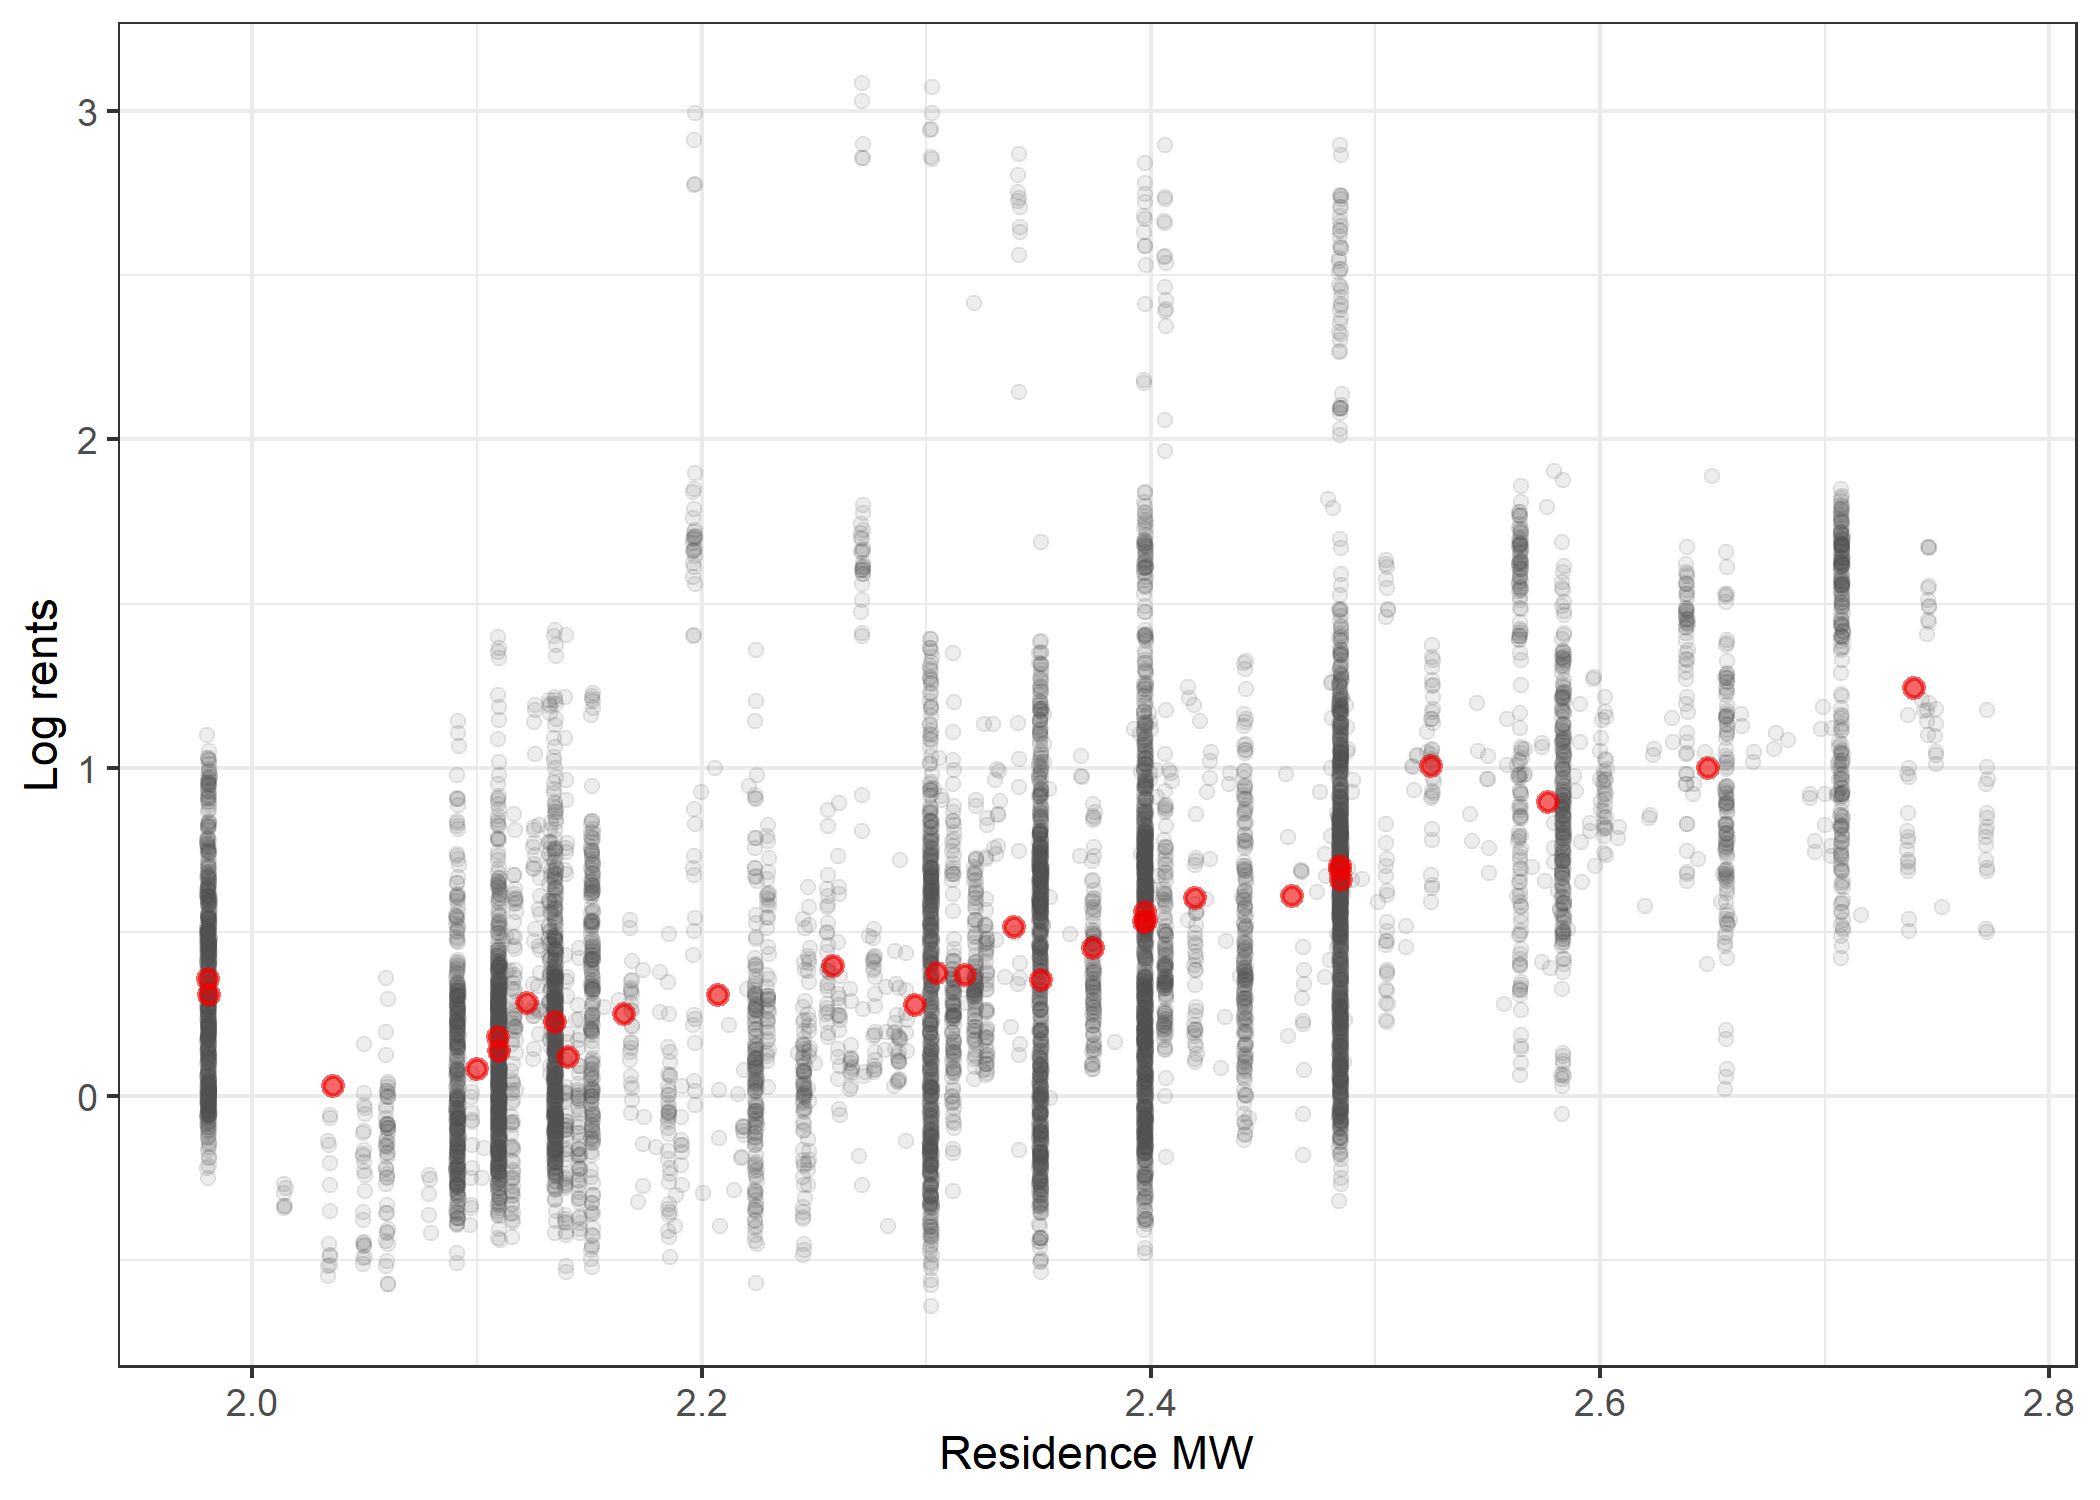
\includegraphics[width = 1\textwidth]
            {plots/cbsa_month_mw_res.png}
    \end{subfigure}\\
    \begin{subfigure}{.7\textwidth}
        \caption{Conditional on ZIP code and workplace MW indicators}
        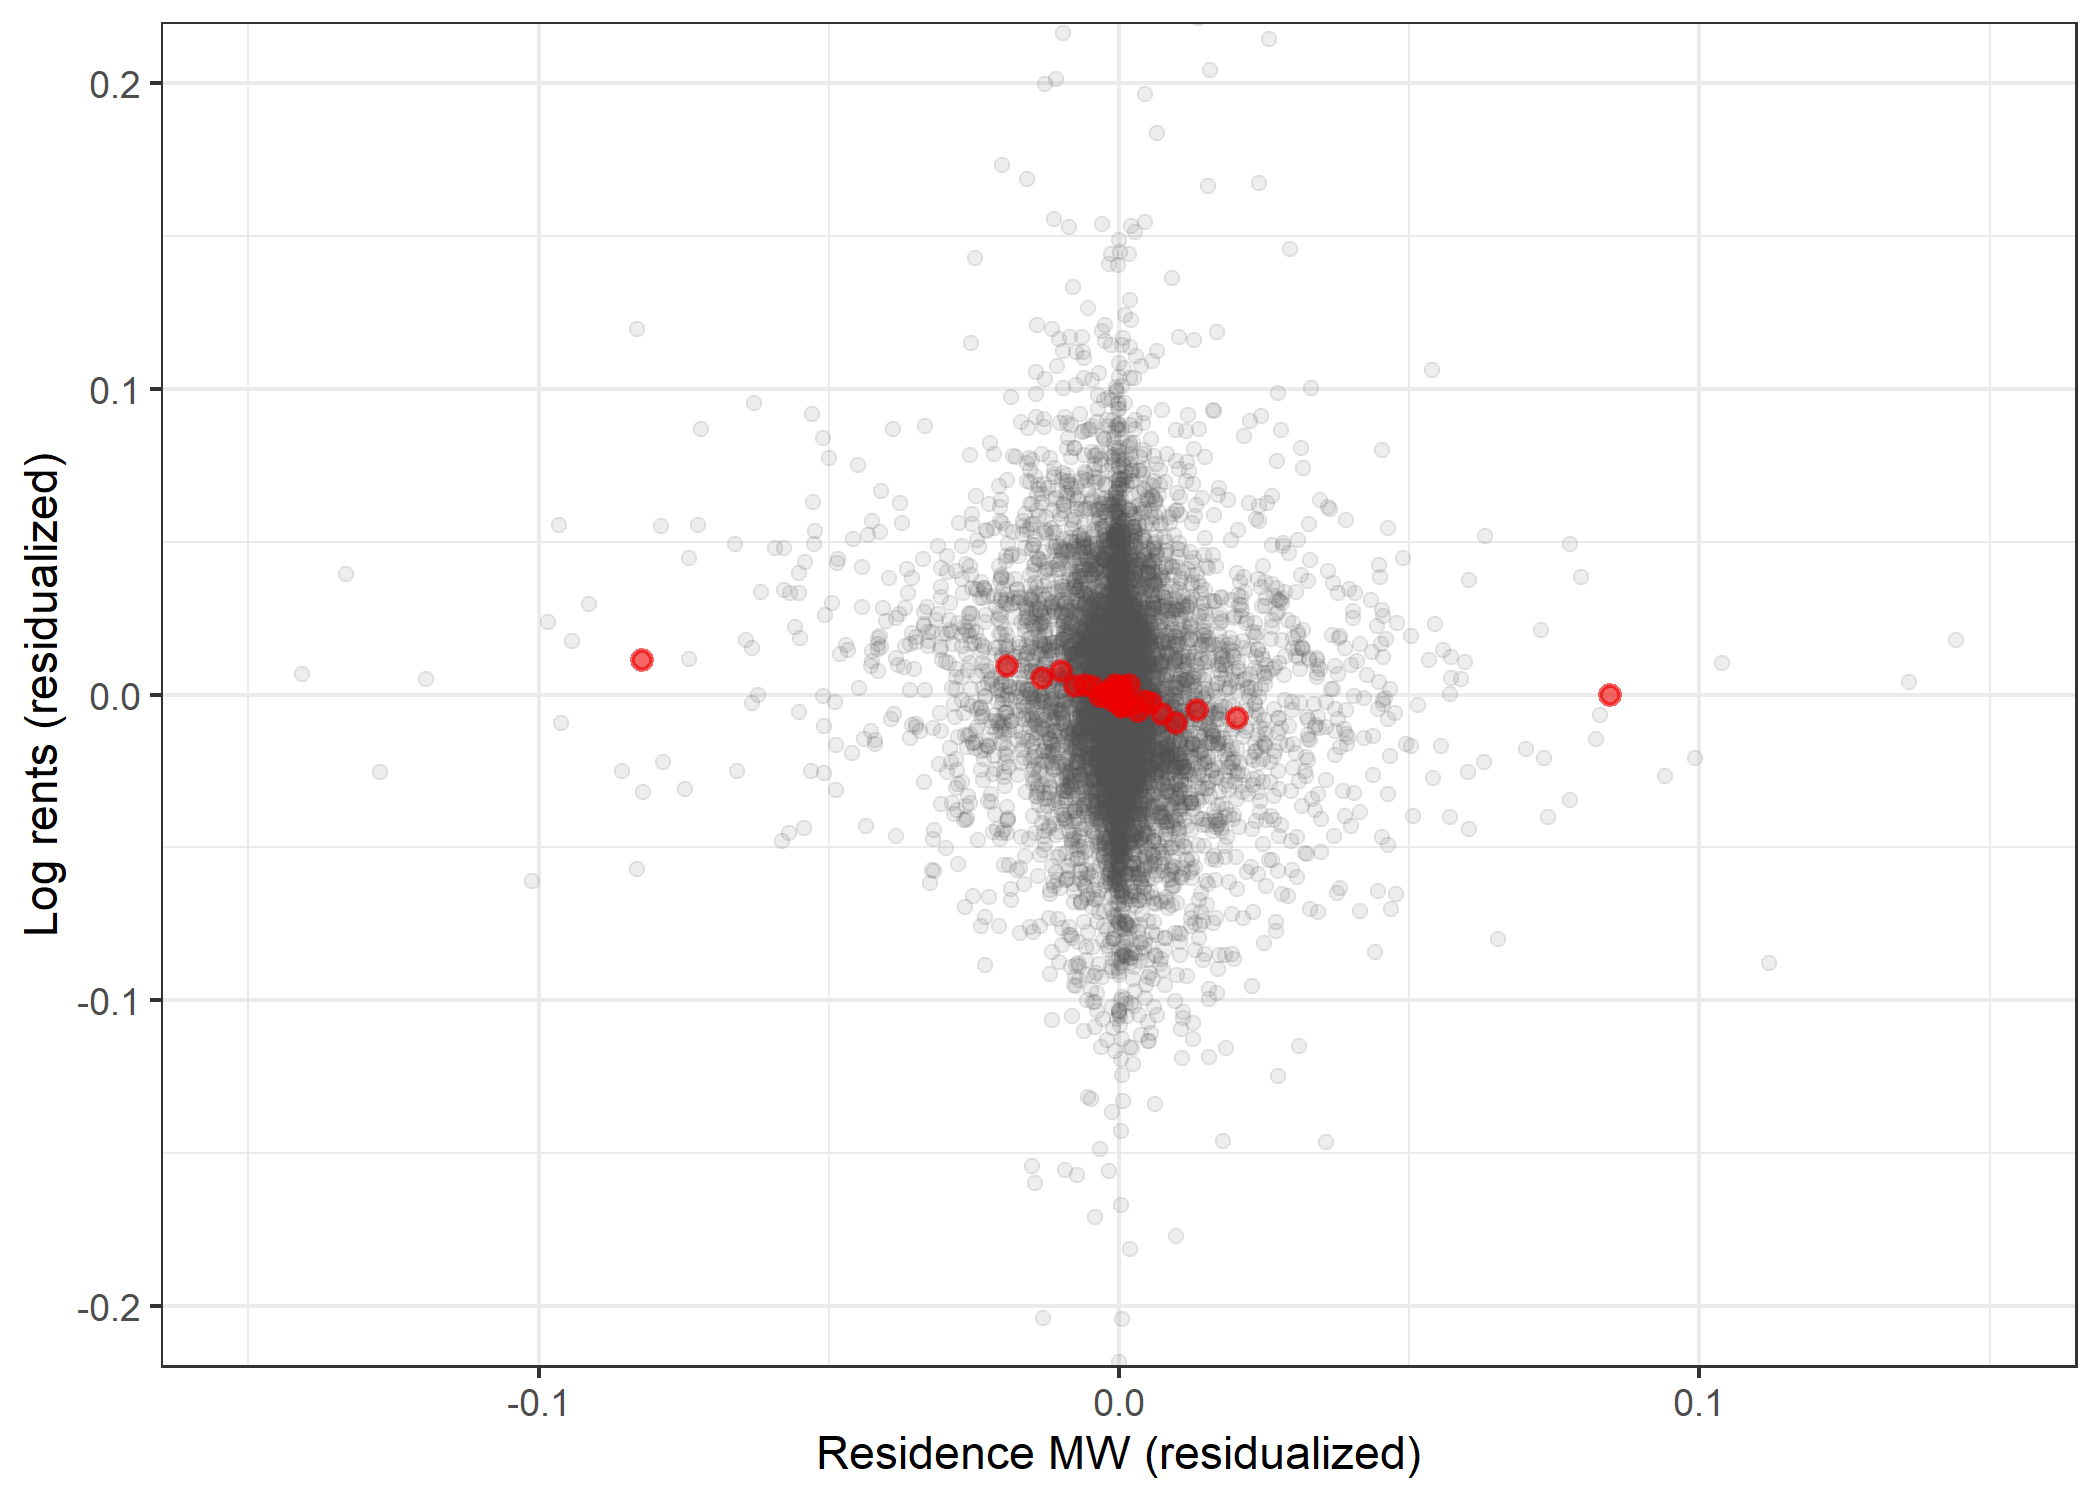
\includegraphics[width = 1\textwidth]
            {plots/cbsa_month_mw_res_resid_mw_wkp_dec.png}
    \end{subfigure}

    \begin{minipage}{.95\textwidth} \footnotesize
        \vspace{3mm}
        Notes: Data are from Zillow and LODES.
        We keep in the sample ZIP code-month observations located in CBSAs 
        where there was some MW increase in the month of interest. 
        Rents correspond to log rents per square foot in the SFCC category.
        The workplace MW measure uses LODES data from the closest prior year.
        The top figure shows the raw relationship between log rents
        and the residence MW.
        The bottom figure shows the same relationship using residuals from 
        regressions on ZIP code indicators and 100 workplace MW indicators.
        Red dots are 30 equally-sized bins of the $x$-axis variable.
        For ease of computation of quantiles, we added a random number between 
        $-.001$ and $.001$ to the residence MW measure in the top figure.
    \end{minipage}
\end{figure}

\end{document}
